\chapter{Resultados}
\label{ch:Resultados}

\section{Processo de AM}
Esta seção descreve a realização do processo de AM, deste a coleta até a apresentação dos dados.
\subsection{Coleta}
Os dados utilizados para a classificação, são referentes a \textbf{Coleta 1 - Tremor de Repouso}, uma vez que esta apresentou os melhores resultados na classificação, já que as outras três coletas apresentaram um alto ruído que acabaram comprometendo os dados. A seguir um pequeno resumo sobre esta coleta.

Foram realizadas três coletas por colaborador, com duração de cinco segundos cada, a disposição dos eletrodos encontra-se no Apêndice \ref{apendicetae}. Os dados do sinal foram armazenadas através da utilização de 4 canais, sendo eles:

\begin{enumerate}
    \item \textbf{CH1}: Extensor radial do longo do carpo direito;
    \item \textbf{CH2}: Flexor superficial dos dedos direito;
    \item \textbf{CH3}: Extensor radial do longo do carpo esquerdo;
    \item \textbf{CH4}: Flexor superficial dos dedos esquerdo.
\end{enumerate}

Estes dados coletados em sEMG em cada canal, foram cedidos no formato \textit{edf}. Sendo que, os grupos consistiam em 14 pessoas no grupo de controle, cada um com três amostras e 14 pessoas no grupo de pessoas com a DP, também com três amostras cada.

\subsection{Processamento dos dados}
Com os dados brutos foi iniciada a etapa de pré-processamento dos dados. Inicialmente utilizou-se como técnica para a filtragem dos dados a FFT, onde se realizou testes nos quatro canais disponíveis, realizando um comparativo da acurácia com e sem a FFT, além de um comparativo sobre a acurácia entre os canais.

Com relação aos dados obtidos em cada canal, como pode ser observado na Figura \ref{fcomparativo1}. Utilizando a FFT obteve-se um bom resultado nos canais \textbf{CH1} com uma precisão média de 78\% e um resultado razoável no \textbf{CH3} com precisão média de 69\%. Já o \textbf{CH4} obteve uma precisão insatisfatória de  59\% de acerto, resultado semelhante ao \textbf{CH2} que teve a precisão de 58\%.


\begin{table}[]
\centering
\begin{tabular}{lccc}
\hline
\multicolumn{4}{c}{Comparativo entre os canais com a FFT.}                                                                \\ \hline
    & \multicolumn{1}{l}{\textbf{Parkinson}} & \multicolumn{1}{l}{\textbf{Controle}} & \multicolumn{1}{l}{\textbf{Média}} \\
CH1 & 86\%                                   & 67\%                                  & \textbf{78\%}                      \\
CH2 & 64\%                                   & 50\%                                  & 58\%                               \\
CH3 & 71\%                                   & 67\%                                  & 69\%                               \\
CH4 & 71\%                                   & 25\%                                  & 59\%                               \\ \hline
\end{tabular}
\caption{Comparativo da precisão entre os canais com a FFT.}
\label{fcomparativo1}
\end{table}


Uma Visão mais detalhada sobre este resultado pode ser observada nas matrizes de confusão na Figura \ref{fcomparativo2} e na Figura \ref{fcomparativo3}. Com relação ao \textbf{CH1} obteve-se uma precisão de 86\% com 14\% de falsos positivos no grupo de DP e uma precisão de 67\% de acerto e 33\% de falsos positivos no grupo de controle. Já o canal \textbf{CH2} obteve um péssimo resultado no grupo de controle com somente 50\% de acerto. 

\begin{figure}[!t]
    \centering
    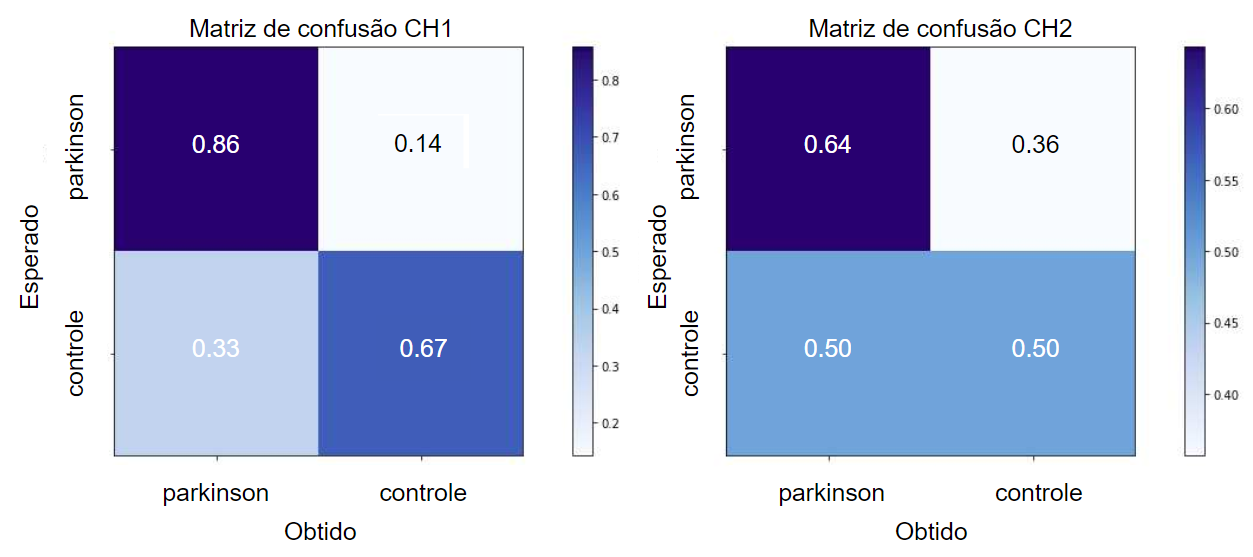
\includegraphics[width=1.1\textwidth]{figuras/1e2.eps}
    \caption{Comparativo entre os canais 1 e 2, com a FFT.}
    \label{fcomparativo2}
\end{figure}

Outro canal que teve um resultado ruim foi o canal \textbf{CH4}, mesmo com 71\% de acerto no grupo com a DP, obteve 75\% de falsos positivos no grupo de controle. Já o \textbf{CH3} obteve um resultado razoável com precisão de 71\% no grupo com DP e e 67\% no grupo de controle.

\begin{figure}[!t]
    \centering
    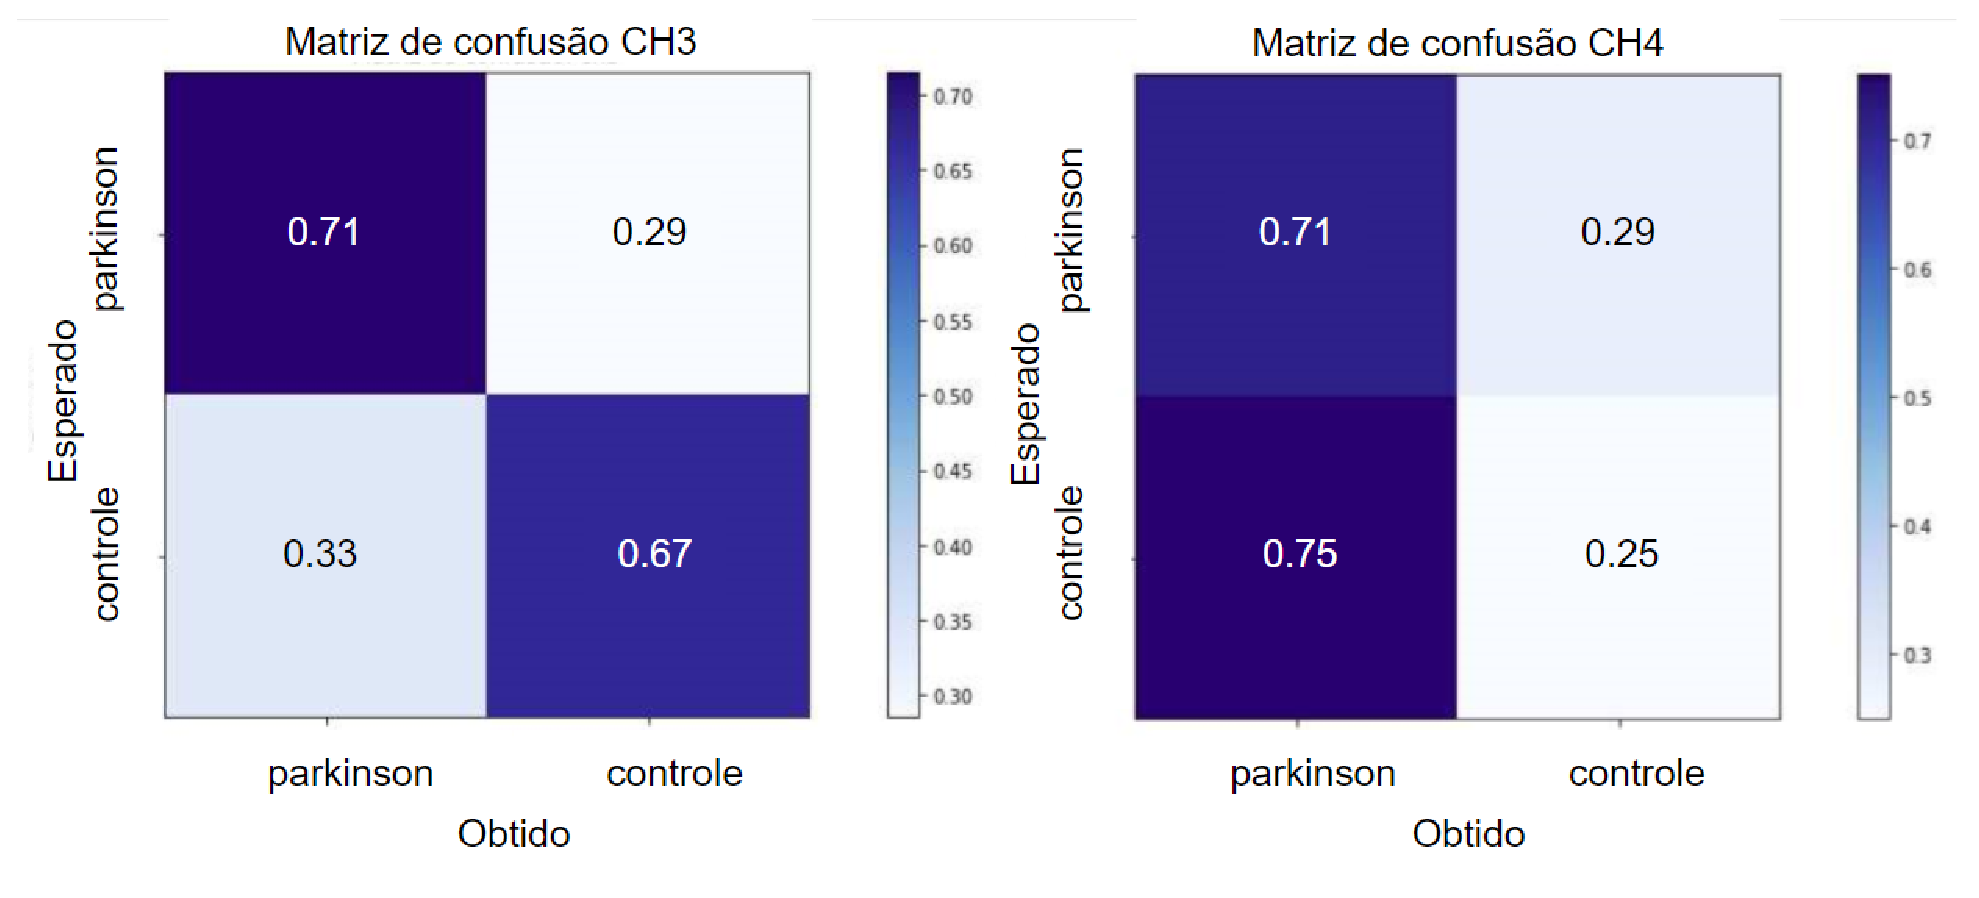
\includegraphics[width=1.1\textwidth]{figuras/3e4.eps}
    \caption{Comparativo entre os canais 3 e 4, com a FFT.}
    \label{fcomparativo3}
\end{figure}


Realizou-se também a aplicação de filtros de frequência, passa-banda, passa-baixa e passa-alta. Porém estes filtros diminuíram a acurácia obtida, como observado na Figura \ref{comesemfiltro}, que exemplifica a matriz de confusão referente ao \textbf{CH1}, assim como normalizou-se os dados em diferentes escalas e do mesmo modo a acurácia caiu. 

Na Figura \ref{comesemfiltro} tem-se que, com a utilização do filtro passa-banda com um total de 11 amostras de pessoas com DP, o sistema conseguiu classificar corretamente 7 amostras ou 64\%, e no grupo de controle classificou-se corretamente 5 amostras de um total de 6 ou 83\%. Com relação aos testes sem a utilização do filtro, obteve-se uma previsão de 90\% no grupo de DP e 71\% no grupo de controle, portanto superior ao testes utilizando o filtro.


\begin{figure}[t]
    \centering
    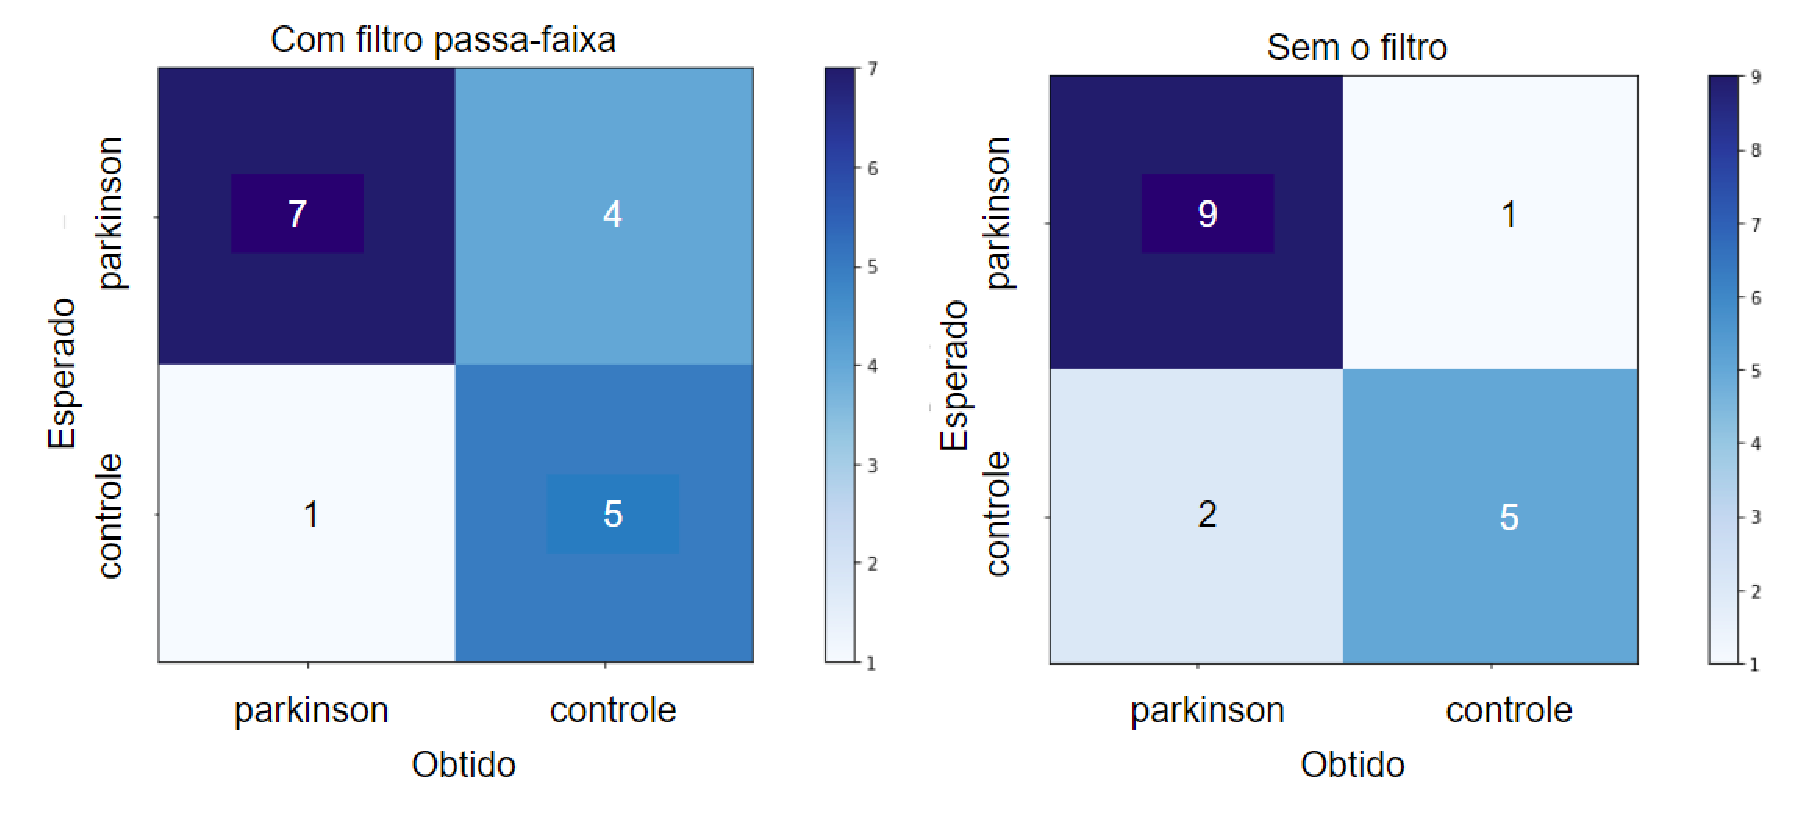
\includegraphics[width=1\textwidth]{figuras/comesemfiltro.eps}
    \caption{Matriz de confusão com o filtro passa-banda e sem o filtro no \textbf{Ch1}.}
    \label{comesemfiltro}
\end{figure}

Também realizou-se a classificação utilizando todos os canais ao mesmo tempo, porém o resultado foi insatisfatório.

Outra técnica de seleção de feature utilizada foi a PCA, com a utilização desta técnica obteve-se uma leve melhora na acurácia, como pode ser observado na Tabela \ref{pcavalidator}, a qual utilizou-se o \textit{cross-validator} para verificar a precisão real do modelo.

Como pode ser observado na Figura \ref{pcavalidator}, com o auxílio do k-fold, pode-se inferir que o \textit{Random Forest} possui uma precisão superior ao SVM, além de que o PCA aumenta a acurácia consideravelmente do modelo.


% Please add the following required packages to your document preamble:
% \usepackage{booktabs}
\begin{table}[]
\centering
\begin{tabular}{@{}lccc@{}}
\toprule
\multicolumn{4}{c}{Comparativo entre os algoritmos com PCA e a FFT.}                                                                                \\ \midrule
                                 & \multicolumn{1}{l}{\textbf{SVM}} & \multicolumn{1}{l}{\textbf{Random Forest}} & \multicolumn{1}{l}{\textbf{KNN}} \\
Somente FFT                      & \textbf{80,76923\%}              & 69,23076\%                                 & 53,84615\%                       \\
FFT com PCA                      & \textbf{84,61538\%}              & 80,76923\%                                 & 53,84615\%                       \\
Somente FFT com Cross-validation & 68\%                             & \textbf{75\%}                              & 59\%                             \\
FFT com PCA e Cross-validation   & 74\%                             & \textbf{79\%}                              & 59\%                             \\ \bottomrule
\end{tabular}
\caption{Comparativo entre os algoritmos do \textbf{Ch1}.}
\label{pcavalidator}
\end{table}




Finalizando a etapa de pré-processamento dos dados, optou-se pela utilização da FFT com o PCA, uma vez que, esta combinação obteve os melhores resultados. Utilizou-se então o \textit{Random Forest} devido a sua acurácia ser levemente superior ao SVM e o consideravelmente superior ao KNN.


\section{Solução de software}
O software pode ser acessado livremente no GitHub, através do seguinte repositório \textbf{https://github.com/SkiNgK/mlModels}, na pasta \textbf{sistema}, divididos em \textit{backend} e \textit{frontend}. Os detalhes referentes a implementação estão descritos nas seções seguintes.

\subsection{Arquitetura}
O documento de Arquitetura encontra-se no anexo \ref{adoarquitetura}.

\subsection{Visão}
O documento de Visão encontra-se no anexo \ref{adocvisao}.

\subsection{Produto}
Os detalhes referentes a construção do produto encontram-se descritos no documento de Visão \ref{adocvisao} e no documento de Arquitetura \ref{adoarquitetura}, a seguir as telas do sistema.


\subsubsection{Pagina inicial}
A figura ~\ref{fighome} exemplifica a página inicial da aplicação, sendo que esta aplicação  conterá somente três páginas. Além da página inicial tem-se a página de pacientes arquivados e a página sobre com as informações relacionadas a metodologia e resultados sobre o processo de Aprendizado de Máquinas utilizado no desenvolvimento da aplicação.

\begin{figure}[!htb]
    \centering
    \includegraphics[width=1\textwidth]{figuras/produto/home.eps}
    \caption{Pagina inicial.}
    \label{fighome}
\end{figure}

\subsubsection{Cadastro de pacientes}
A figura ~\ref{figcadastro} refere-se ao cadastro de pacientes. Nesta tela inserem-se os seguintes itens, todos obrigatórios:
\begin{itemize}
    \item Nome completo;
    \item Idade;
    \item Sexo;
    \item Arquivo sEMG em formato \textit{edf}.
\end{itemize}

\begin{figure}[!htb]
    \centering
    \includegraphics[width=1\textwidth]{figuras/produto/cadastro.eps}
    \caption{Cadastro das pacientes.}
    \label{figcadastro}
\end{figure}

\subsubsection{Edição de pacientes}
Para realizar a edição dos dados de um paciente, como demonstrado na figura ~\ref{figcadastro}, ao pressionar o botão \textbf{EDITAR} na aba de opções é aberto um \textit{modal} contendo as informações do paciente para a alteração. Para alterar o arquivo sEMG é necessário clicar em alterar arquivo, o qual após adicionado substitui o antigo.

\begin{figure}[!htb]
    \centering
    \includegraphics[width=1\textwidth]{figuras/produto/editar.eps}
    \caption{Editar dados dos pacientes.}
    \label{figeditar}
\end{figure}

\subsubsection{Avaliar pacientes}
Para avaliar um paciente recém inserido, é necessário clicar no botão \textbf{AVALIAR}, como na figura ~\ref{figavaliar}.
\begin{figure}[!htb]
    \centering
    \includegraphics[width=1\textwidth]{figuras/produto/avaliar.eps}
    \caption{Avaliar pacientes.}
    \label{figavaliar}
\end{figure}

\subsubsection{Pesquisar pacientes}
Para pesquisar por qualquer um dos itens das colunas, basta clicar no ícone de pesquisa como na figura ~\ref{figpesquisar} e inserir o termo da pesquisa.
\begin{figure}[!htb]
    \centering
    \includegraphics[width=1\textwidth]{figuras/produto/pesquisar.eps}
    \caption{Pesquisar itens pelas colunas.}
    \label{figpesquisar}
\end{figure}

\subsubsection{Pesquisar pacientes}
Também é possível executar outras opções como \textit{download} da tabela, impressão e exibir colunas. Como pode ser observado na figura ~\ref{figpesquisar}.
\begin{figure}[!htb]
    \centering
    \includegraphics[width=1\textwidth]{figuras/produto/outrasop.eps}
    \caption{\textit{Download} da tabela, impressão e exibir colunas.}
    \label{figoutrasop}
\end{figure}

\subsubsection{Pagina arquivados}
Para exibir os itens arquivados, clica-se na aba \textbf{ARQUIVADOS}, como na figura ~\ref{farquivados}.
\begin{figure}[!htb]
    \centering
    \includegraphics[width=1\textwidth]{figuras/produto/arquivados.eps}
    \caption{\textit{Download} da tabela, impressão e exibir colunas.}
    \label{farquivados}
\end{figure}

\subsubsection{Página sobre}
A página sobre exibe as informações referentes ao trabalho, Figura ~\ref{fsobre}.
\begin{figure}[!htb]
    \centering
    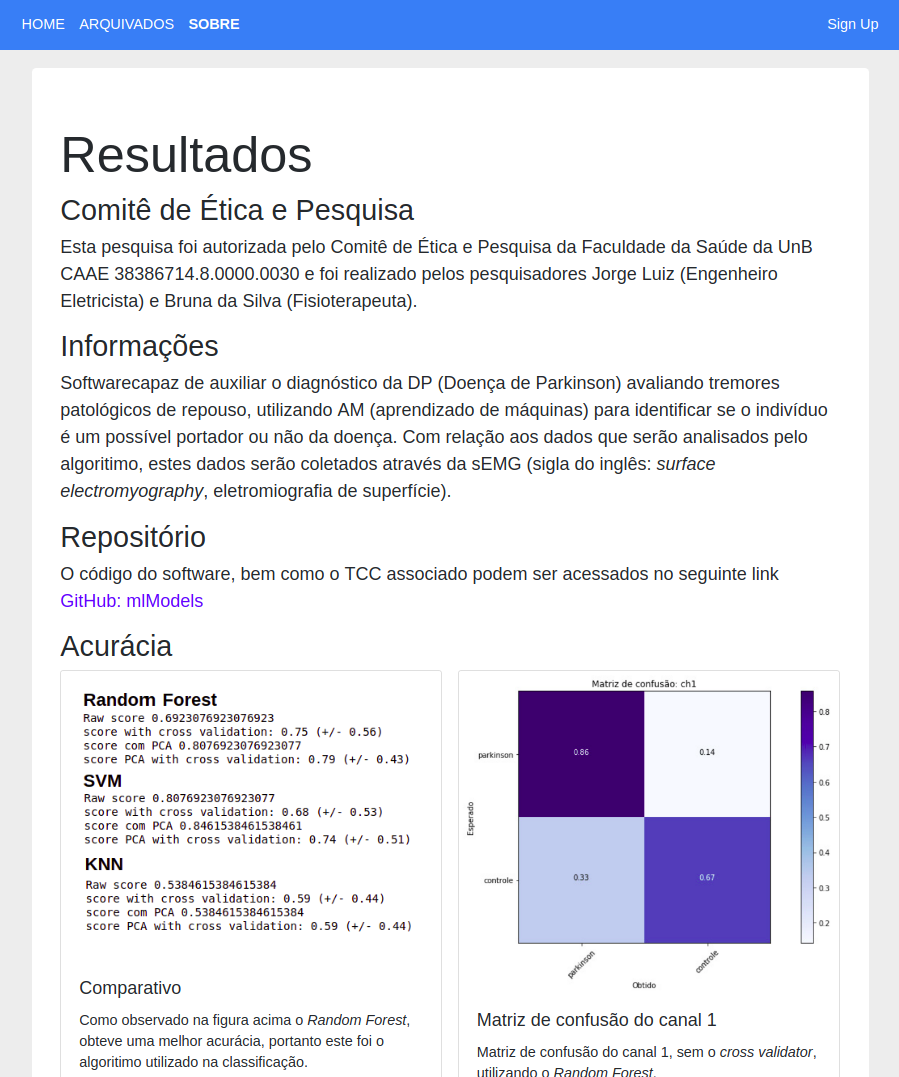
\includegraphics[width=1\textwidth]{figuras/paginasobre.eps}
    \caption{informações sobre o projeto, na página Sobre.}
    \label{fsobre}
\end{figure}

\section{Passos futuros e considerações finais}
   Conseguiu-se atingir os objetivos propostos, provando que é possível classificar com uma boa acurácia a doença de Parkinson utilizado Aprendizado de Máquinas. Com aproximadamente 79\% de precisão,isto considerando o baixo nível de amostras, 36 no total. Além disto, foi desenvolvida uma software totalmente operacional, onde um profissional da saúde consegue classificar facilmente uma pessoa em alta ou baixa probabilidade de possuir a DP.

   Como passos futuros, é desejável a realização de mais coletas, com a finalidade de aumentar as amostras de treinamento e consequentemente aumentar a acurácia na classificação da DP. Também é desejável a realização de uma anamnese mais detalhada.
